% 1. human-made video
% 2. paper
% Wan2.1
% PPTAgent

% pptx / beamer / beamer + debug / bearm +debug+tree search

% user study

% IP: ask a reasonable question

\vspace{-0.5\baselineskip} 
\section{Experiments}
\vspace{-0.4\baselineskip} 
\subsection{Baseline and Settings}
\vspace{-0.4\baselineskip} 
We evaluate three categories of baselines: \textbf{(i)} End-to-end Methods~\cite{wan,deepmind2025veo3}, where natural video generation models produce the presentation video directly from a prompt generated by paper; \textbf{(ii)} Multi-Agent Frameworks~\cite{shi2025presentagent,zheng2025pptagent}, which combine slide generation with text-to-speech generation and compose them into a presentation video; and \textbf{(iii)} {\agent}, our method and its variants. For the VLM and VideoLLM, we choose \textit{GPT-4.1} and \textit{Gemini-2.5-Flash}, respectively, for a favorable efficiency and performance trade-off. We perform inference using eight NVIDIA RTX A6000 GPUs.


% End-to-end, multi-agent, slide-agent, ours
% \vspace{-1\baselineskip} 
\vspace{-0.4\baselineskip} 
\subsection{Main Results}
% \kevin{highlight exps as showui}
\vspace{-0.5\baselineskip} 
\textbf{Meta Similarity.} We evaluate the alignment of the generated slides, subtitles, and speech with corresponding human-authored ones. For speech, we randomly sample a 10-second audio segment from the video generated by each method and compute the cosine similarity between its embeddings~\cite{audio_embedding} and those of the author’s speech. As shown in Table~\ref{tab:main_result}, {\agent} attains the highest scores in both speech and content similarity, demonstrating that its outputs \textbf{align most closely with human creation} among all baselines. We attribute this performance to personalized TTS and our slide-generation design: \textbf{(i)} adopting \textit{Beamer}, which provides formal, academically styled templates while \LaTeX{} automatically arranges content within each slide; and \textbf{(ii)} a tree search visual choice layout refinement that further enforces fine-grained slide layouts as commonly observed in human-authored slides.

\vspace{-0.4\baselineskip} 
\textbf{PresentArena.} We compare the presentation videos generated by each method against the human-made videos. As an automatic evaluator, we prompt the VideoLLMs as a judge to determine which presentation is better with respect to clarity, delivery, and engagement. As shown in Table~\ref{tab:main_result}, {\agent} attains the highest pairwise winning rate among all baselines, indicating that our method produces presentation videos with \textbf{superior overall perceived quality}. Notably, {\agent} outperforms its variants without the talker and cursor by 1.8\%, highlighting the gains introduced by these components and implying that the VideoLLM \textbf{favors presentation videos with a talker presenting}.

% \kevin{\textbf{Talkinghead} XXXX}

\vspace{-0.4\baselineskip} 
\textbf{PresentQuiz.} To assess information coverage, we conduct a VideoQA evaluation. Following prior work on posters~\cite{pang2025paper2poster}, we construct QA sets by prompting an LLM to generate questions targeting (i) fine-grained details and (ii) higher-level understanding of the paper. The videos and QA sets are then fed into a VideoLLM to conduct the quiz.
As shown in Table~\ref{tab:main_result}, {\agent} achieves superior performance across both aspects, outperforming HumanMade and PresentAgent despite shorter video length. This indicates that {\agent} produces videos that are \textbf{more informative within shorter durations}. Furthermore, the absence of the talker or cursor results in performance degradation, as the cursor trajectory  potentially \textbf{guides the attention and supports accurate grounding of the key contents} for the VideoLLMs during inference, referring to Table~\ref{table:cursor} for more details.

\vspace{-0.4\baselineskip} 
\textbf{IP Memory.} We evaluate the degree to which the generated presentation videos facilitate audience retention of the work, thereby assessing their memorability and lasting impact. {\agent} achieves the highest recall accuracy. This improvement mainly stems from the inclusion of an engaging talker with the author’s figure and voice, which \textbf{significantly helps the audience retain the video content}.

% {\agent}’s gains stem from our slide-generation design and our principled cursor-trajectory synthesis, which together guide attention and enable accurate grounding of key content for the VideoLLMs. Although PresentAgent attains slightly higher unpenalized accuracy, its length-penalized score is markedly lower owing to the excessive duration of its generated videos compared with human-made videos.

\begin{wrapfigure}[15]{r}{0.35\textwidth} % 12=大致占用的行数,可调 8~16
  \vspace{-0.8\baselineskip}              % 往上顶,避免与上一行留白
  \centering
  \small
  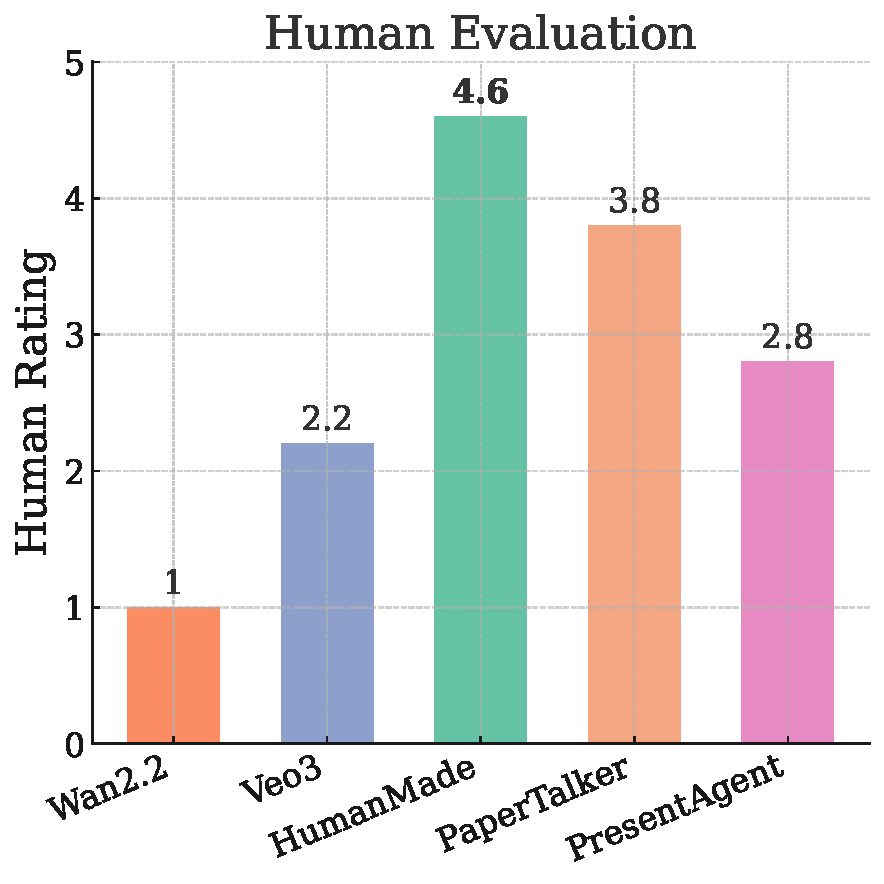
\includegraphics[width=\linewidth]{figure/human_evaluation_bar.pdf}
  \captionsetup{skip=0pt}                 % 图↔标题更紧
  \caption{\small \textbf{Human evaluation}. We randomly sample the generated results from ten papers for evaluation.}
  \label{fig:human_eval}
  %\vspace{-1\baselineskip}              % 与后续正文再贴近
  %\vspace{-0.5\baselineskip}
\end{wrapfigure}
\vspace{-0.3\baselineskip} 
\textbf{Human Evaluation.}
To further assess the quality of the generated presentations from the user perspective, we conducted a human evaluation in which ten participants were provided with each paper along with its corresponding presentation videos generated by different methods. Participants were asked to rank the videos according to their preferences($1\text{(worse)}-5\text{(best)}$).
As shown in Figure~\ref{fig:human_eval}, human-made videos achieve the highest score, with {\agent} ranking second and outperforming all other baselines. This demonstrates that presentation videos generated by {\agent} \textbf{gain consistently favor from human users} over other baselines and \textbf{comparable to human-made}.

\begin{table*}[t]
  \centering
  \setlength{\tabcolsep}{4pt}
  \footnotesize
  \caption{\textbf{Detailed evaluation result of {\bench} across three baselines.} $\text{PaperTalk}^{*}$ represents a simple version without presenter and cursor. \textbf{Bold} and \underline{Underline} indicates the best and the second.}
  \label{tab:main_result}

  \begin{tabular*}{\linewidth}{l c c c c c c c}

    \toprule
    \multirow{2}{*}{Method} &
    \multicolumn{2}{c}{Similarity$\uparrow$} &
    \multirow{2}{*}{Arena$\uparrow$} &
    \multicolumn{2}{c}{PresentQuiz Acc.$\uparrow$} &
    \multirow{2}{*}{IP Memory$\uparrow$} &
    \multirow{2}{*}{Avg. Duration(s)}\\
    \cmidrule(lr){2-3}\cmidrule(lr){5-6}
    & Speech & Content & & Detail & Under.\\
    \midrule
    HumanMade & \textbf{1.00} & \textbf{5.00}  & \textbf{50.0\%}  & 0.738  & 0.908  & - & 375.15\\
    \midrule
    \rowcolor{gray!20} Wan2.2~\cite{wan} & NA & NA & 1.1\% & 0.251 & 0.551 & 11.5\% & 4.00\\
    \rowcolor{gray!20} Veo3~\cite{deepmind2025veo3} & 0.133 & NA & 1.2\% & 0.367 & 0.585 & 31.3\% & 8.00\\
    PresentAgent\textsubscript{QWEN}~\cite{shi2025presentagent} & - & 0.24 & - & - & - & - & - \\
    PresentAgent\textsubscript{GPT4.1}~\cite{shi2025presentagent} & 0.045 & 1.47 & 2.0\% & 0.548 & 0.654 & 12.5\% & 430.20\\
    \midrule
    PaperTalk\textsubscript{QWEN} & - & 1.66 & - & - & - & - & - \\
    $\text{PaperTalk\textsubscript{GPT4.1}}^{*}$ & \underline{0.646} & \underline{1.97} & 15.2\% & \underline{0.835}  & \underline{0.949} & \underline{37.5\%} & 234.36 \\
    PaperTalk\textsubscript{GPT4.1} & \underline{0.646} & \underline{1.97} & \underline{17.0}\% & \textbf{0.842}  & \textbf{0.951} & \textbf{50.0\%} & 234.36\\
    \bottomrule
  \end{tabular*}
\end{table*}
\vspace{-0.4\baselineskip}   


\vspace{-0.4\baselineskip} 
\subsection{Qualitative Analysis}
\vspace{-0.4\baselineskip} 
\begin{wraptable}[6]{r}{0.55\textwidth}
  \vspace{-1.8\baselineskip} 
  \centering
  \tablesize
  \caption{\textbf{Generation cost for each method.}}
  {
  \setlength{\tabcolsep}{3pt}
  \begin{tabular}{lccc}
    \toprule
    Method & Token (K) $\downarrow$ & Time (min.)$\downarrow$ & Cost (\text{\$})$\downarrow$ \\
    \midrule
    Veo3~\cite{deepmind2025veo3} & NA & \textbf{0.4} & 1.667 \\
    Wan2.2~\cite{wan} & NA & 8.1 & 0.280 \\
    \hline
    PresentAgent~\cite{shi2025presentagent} & 241 & 39.5 & 0.003  \\
    PaperTalker (w/o Talker) &  \textbf{62} & 15.6 & \textbf{0.001}\\    
    PaperTalker (w/o Par.) & \textbf{62} & 287.2 & \textbf{0.001}\\
    PaperTalker & \textbf{62} & 48.1 \textbf{(6$\times$)} & \textbf{0.001} \\
    \bottomrule
  \end{tabular}
  }
  \label{table:cost}
  \vspace{-2\baselineskip} 
\end{wraptable}
As shown in Figure~\ref{fig:compare}, {\agent} produces presentation videos that \textbf{most closely align with the human-made} ones. While Veo3~\cite{deepmind2025veo3} renders a high-quality speaker in front of the screen, it is constrained by short duration (\textit{e.g.}, 8s) and blurred text. Besides, PresentAgent\cite{shi2025presentagent} typically suffers from the absence of the presenter and slide-design errors (\textit{e.g.}, overflow, incorrect title, incomplete author lists, and institutions).




% table1 comparion, similarity(audio, content), video qa acc, acadimact IP

% \usepackage{booktabs}
% \usepackage{multirow}



% ablation: cursor accuary



% 不同的LLM/VLM
% Layout refinement 
%1) multi-turn 
%2) single turn (single/multi)
% \vspace{-1\baselineskip} 
\vspace{-0.4\baselineskip} 
\subsection{Key Ablations}
\vspace{-0.4\baselineskip} 
%\noindent\textbf{Is Talking Head Necessary?} In presentation videos, the presence of a presenter substantially affects audience engagement. Empirically, the PresentArena results in Table~\ref{tab:main_result} show {\agent} outperforming its no-presenter, no-cursor variant PaperTalker* by more than 10\%, implying that the VideoLLM prefers presentation videos which includes a presenter. 
%\kevin{PaperTalker*} \kevin{add exactly number}
% \kevin{Human eval;}
\begin{wraptable}[3]{r}{0.4\textwidth} % 右侧;宽度可调;[6] 是预估占用行数
  \vspace{-2\baselineskip}               % 可选:向上收一点
  \tablesize
  \centering
    \caption{\textbf{Ablation study on cursor.}}
  \begin{tabular}{lc}
    \toprule
    Method & Accuracy$\uparrow$ \\
    \midrule
    PaperTalker (w/o Cursor) &  0.084 \\
    PaperTalker &\textbf{0.633} \\
    \bottomrule
    \label{table:cursor}
  \end{tabular}
\end{wraptable}
\noindent\textbf{What benefits are brought by Cursor Highlight?} 
Motivated by the observation that a cursor typically helps audiences locate the relevant region, we hypothesize that a visible cursor, by providing an explicit spatial cue, facilitates content grounding for VLMs. To evaluate this, we design a localization QA task: for each subtitle sentence and its corresponding slide, a VLM generates a four-option multiple-choice question about the sentence’s corresponding position on the slide. The VLMs are then prompted to answer using slide screenshots, with or without the cursor, and accuracy is measured as the metric. As shown in Table~\ref{table:cursor}, the accuracy is much higher with the cursor highlight, corroborating its \textbf{importance for the audience's visual grounding accessibility} of presentation videos. 

\begin{wraptable}[8]{r}{0.6\textwidth} % [10] 行数可调, r=右侧, 宽度自己调
 \vspace{-1\baselineskip} 
  \centering
  \tablesize
  \caption{\textbf{Evaluation result on slide quality}.}
  {
  \setlength{\tabcolsep}{1pt} % 默认是6pt,这里改小
  \begin{tabular}{lccc}
    \toprule
    Method & Content ($\uparrow$) & Design ($\uparrow$) & Coherence ($\uparrow$) \\
    \midrule
    HumanMade & \textbf{4.43} & \textbf{2.85} & 2.73 \\
    \midrule
    $\text{PPTAgent}_\text{Qwen7B}$~\cite{zheng2025pptagent} & 3.43 & 1.57 & 1.29 \\
    $\text{PaperTalker}_\text{Qwen7B}$ & 4.00 & 2.53 & \underline{3.11} \\
    \midrule
    $\text{PPTAgent}_\text{GPT4.1}$~\cite{zheng2025pptagent} & 4.07 & 2.02 & 2.06 \\
    $\text{PaperTalker}_\text{GPT4.1}$(w/o Tree Search) & 4.33 & \underline{2.73} & \textbf{3.84} \\
    $\text{PaperTalker}_\text{GPT4.1}$ & \underline{4.34} & \textbf{2.85} & \textbf{3.84} \\
    \bottomrule
  \end{tabular}
  }
  \label{tab:slide_quality}
\end{wraptable}
\noindent\textbf{How does tree search visual choice improve slide quality?} To assess the contribution of the tree-search visual choice module, we conduct an ablation experiment, as shown in Table~\ref{tab:slide_quality}. In line with prior work on slide generation~\cite{zheng2025pptagent}, we assess the generated slides using a VLM on a 1–5 scale across content, design, and coherence. The results show a pronounced decline in design quality when layout refinement is removed, highlighting \textbf{the tree-search visual choice module as a key component for slide creation} (\ie~resolving overfull issues), referring to Figures~\ref{fig:tree_vis} for visualization.

\begin{figure}
    \centering
    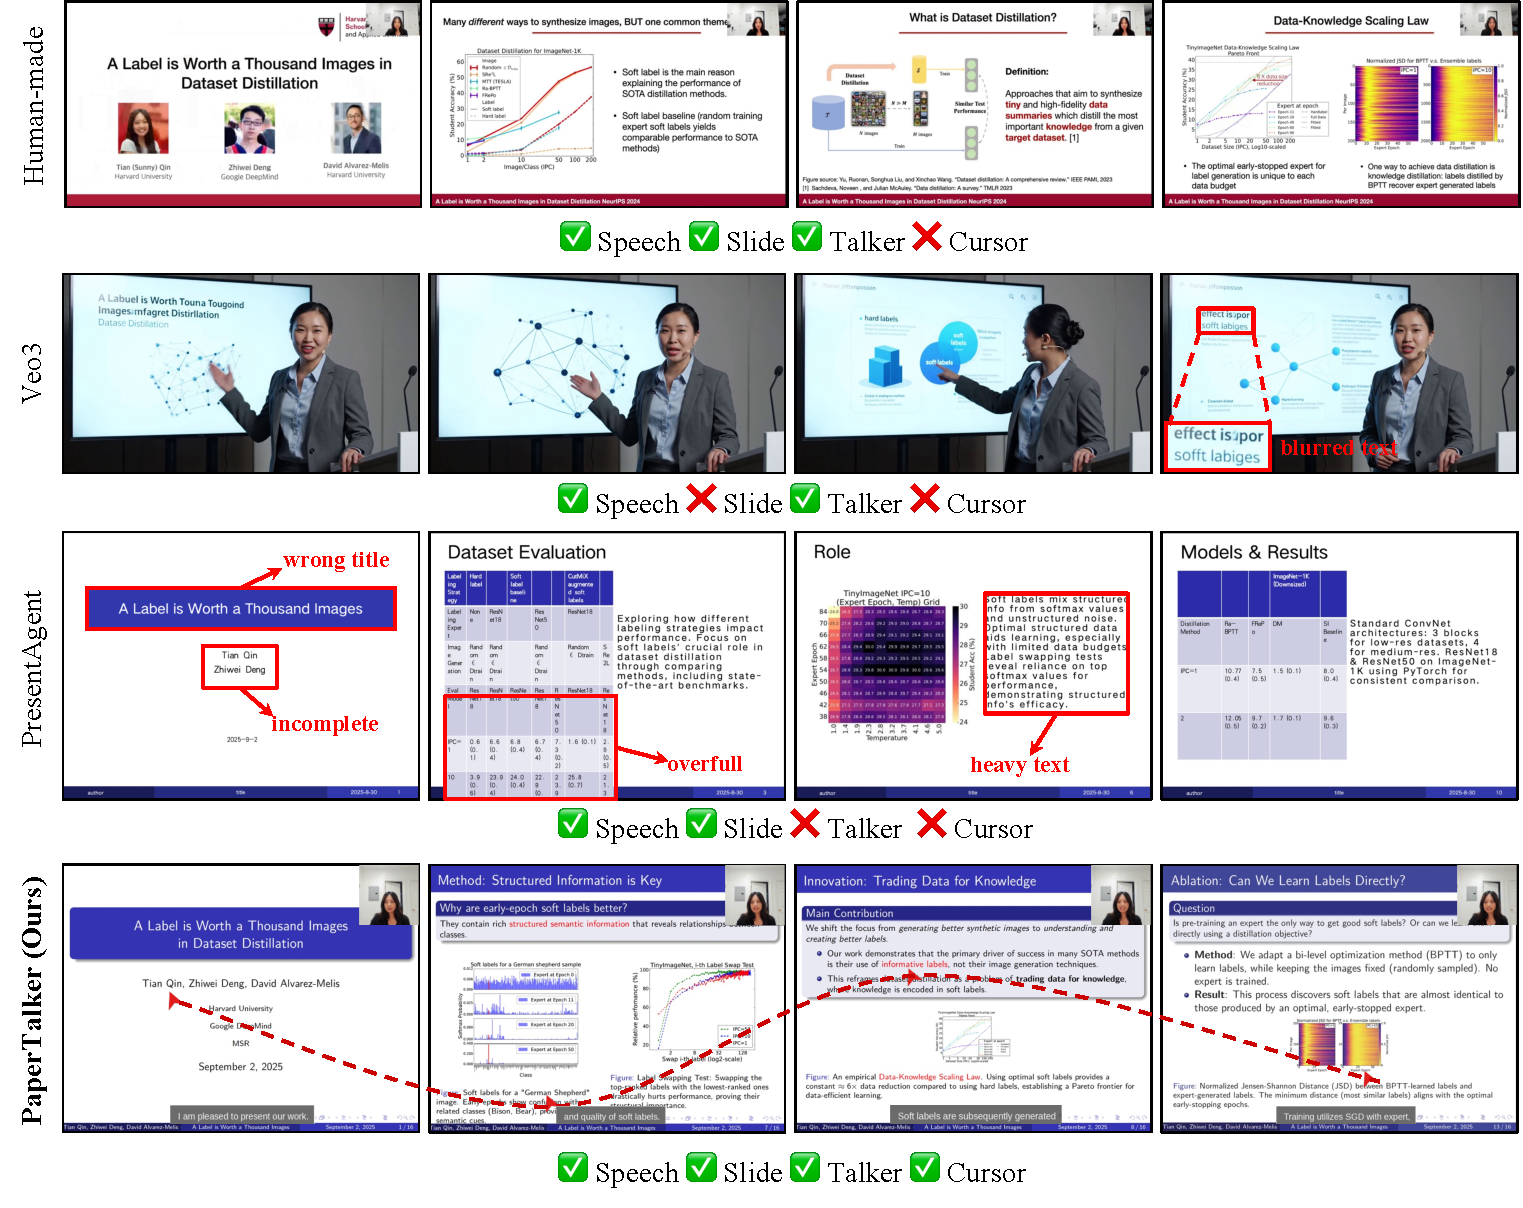
\includegraphics[width=\linewidth]{figure/vis.pdf}
    \captionsetup{skip=0pt}  
    \caption{\textbf{Visualization of generated results.} {\agent} produces presentation videos with rich, fine-grained slide content, accurate cursor grounding, and an engaging talker; in contrast, Veo3~\cite{deepmind2025veo3} yields blurred text and incomplete information coverage, while PresentAgent~\cite{shi2025presentagent} produces text-heavy slides and suffers from overfull layout issues and inaccurate information (\textit{e.g.}, title and institutions).}
    \label{fig:compare}
    \vspace{-0.2\baselineskip} 
\end{figure}
%\kevin{same as aboveww}